\textbackslash{}chapter\{Hamilton--Jacobi Theory\}
\textbackslash{}label\{ch:6\}

6.1
The Hamilton--Jacobi equation
\section*{6.1  The Hamilton--Jacobi equation}

A dynamical problem is solved when we determine relationships for the generalized coordinates and momenta in terms of the initial conditions and the time.
The initial conditions can be expressed as q0 and p0, by which we mean the
constant values of the coordinates (qi) and the momenta (pi) at time t = 0.
The solution of the mechanical problem is the set of relationships
q = q(q0, p0, t),
(6.1)
p = p(q0, p0, t).
These equations can be considered to be a set of transformation equations
between the canonical variables q, p and a new set q0, p0. Finding a solution
to the mechanical problem is equivalent to finding the transformation from q, p
to q0, p0. But q0, p0 are constants; therefore we need to find a transformation
from the canonical variables (q, p) to a set of variables which are constants.
We now show how this can be done.
A canonical transformation takes us from the Hamiltonian H = H(p, q, t)
to the transformed Hamiltonian K = K(P, Q, t), where
$\textbackslash{}dot Q\_i = \textbackslash{}partial K
\textbackslash{}partial Pi
,
$\textbackslash{}dot P\_i = -\textbackslash{}partial K
\textbackslash{}partial Qi
and
K = H + \textbackslash{}partial F
\textbackslash{}partial t .
If the new variables are constants we have $\textbackslash{}dot Q\_i = 0 and $\textbackslash{}dot P\_i = 0. (We want
the ``new'' variables to be the constant initial values of the coordinates and
momenta.) The requirement that the new variables be constant is guaranteed
quite simply by requiring that K be a constant. In fact, if we set K = 0, then
obviously $\textbackslash{}dot Q\_i = 0 and $\textbackslash{}dot P\_i = 0. Setting K = 0 yields
H + \textbackslash{}partial F
\textbackslash{}partial t = 0.
(6.2)
This is a differential equation that can be solved for F. (Recall that F is the
generating function for the canonical transformation.)
We shall chose F to have the form F = F2(q, P, t). This is a reasonable
choice because this generating function takes us from p to P and from q to Q.
You will also recall that this is the basis for the infinitesimal contact transformations that took us from q and p at one time to q and p at some other time.

Hamilton--Jacobi theory
We previously denoted this generating function by F2, but now, for historical
reasons, we shall denote it by S. We do not (yet) know the functional form of
S, but we do know that
S = S(q, P, t).
In Hamilton--Jacobi theory, the function S is called Hamilton's principal
function.
By Equations (5.14)
pi = \textbackslash{}partial S
\textbackslash{}partial qi
,
(6.3)
Qi = \textbackslash{}partial S
\textbackslash{}partial Pi
,
K = H + \textbackslash{}partial S
\textbackslash{}partial t .
If we can determine S, then we will be able to generate the transformation
equations (6.1) and the problem is solved.
Writing (6.2) in terms of S yields the following relationship
H(q1, . . . , qn; p1, . . . , pn; t) + \textbackslash{}partial S
\textbackslash{}partial t = 0.
But pi = \textbackslash{}partial S
\textbackslash{}partial qi , so we can write
H(q1, . . . , qn; \textbackslash{}partial S
\textbackslash{}partial q1
, . . . , \textbackslash{}partial S
\textbackslash{}partial qn
; t) + \textbackslash{}partial S
\textbackslash{}partial t = 0.
(6.4)
This is a partial differential equation for S. It is called the Hamilton--Jacobi
equation. Given the functional form of H it can be solved for S.
Recall that the new variables P and Q are the constant initial conditions. To
emphasize this, one usually writes \textbackslash{}alpha i for Pi and \textbackslash{}beta i for Qi. Then,
S = S(qi, \textbackslash{}alpha i, t).
By Equations (6.3)
pi = \textbackslash{}partial S
\textbackslash{}partial qi
= \textbackslash{}partial S(qi, \textbackslash{}alpha i, t)
\textbackslash{}partial qi
,
(6.5)
and
\textbackslash{}beta i = Qi = \textbackslash{}partial S
\textbackslash{}partial \textbackslash{}alpha i
= \textbackslash{}partial S(qi, \textbackslash{}alpha i, t)
\textbackslash{}partial \textbackslash{}alpha i
.
(6.6)
If Equation (6.6) can be inverted we obtain
qi = qi(\textbackslash{}alpha i, \textbackslash{}beta i, t).
(6.7)

6.2
The harmonic oscillator -- an example
Plugging (6.7) into (6.5) gives
pi =
\textbackslash{}partial
\textbackslash{}partial qi
S(qi(\textbackslash{}alpha i, \textbackslash{}beta i, t), \textbackslash{}alpha i, t),
or
pi = pi(\textbackslash{}alpha i, \textbackslash{}beta i, t).
(6.8)
Equations (6.7) and (6.8) are the desired solution to the dynamical
problem.
\begin{exercise}
Exercise 6.1 Write the Hamilton--Jacobi equation for a free particle.
\end{exercise}

\begin{exercise}
Exercise 6.2 Determine Hamilton's principal function for a free particle.
\end{exercise}

\section*{6.2  The harmonic oscillator -- an example}

As an example of the use of Hamilton--Jacobi theory, let us apply it to the harmonic oscillator problem. Recall that the Hamiltonian for the harmonic oscillator (see Equation 5.19) can be written as
H = 1
2m

p2 + m2\textbackslash{}omega 2q2
,
where \textbackslash{}omega  = \textbackslash{}sqrtk/m. Since H does not contain the time t explicitly, H is a
constant and in this case we know it is equal to the total energy (H = E).
The Hamilton--Jacobi equation (6.4) for this problem is fairly simple because
the Hamiltonian does not depend on time and we can separate variables,
writing
2m
\textbackslash{}partial S
\textbackslash{}partial q
+ m2\textbackslash{}omega 2q2

= -\textbackslash{}partial S
\textbackslash{}partial t .
Integrating both sides gives us a function S having the form
S(\textbackslash{}alpha , q, t) = W(\textbackslash{}alpha , q) + V (\textbackslash{}alpha , t),
where \textbackslash{}alpha  is a constant. If such a separation is possible -- and it often is
possible -- the partial differential equation can be solved reasonably easily. If
such a separation cannot be carried out, the Hamilton--Jacobi technique is not
a useful computational tool. As is often the case with partial differential equations, one assumes the separation is possible, then checks to see if the solution
obtained obeys the differential equation and the boundary conditions.

Hamilton--Jacobi theory
Plugging the separated expression for S into the Hamilton--Jacobi equation
we obtain
2m
\textbackslash{}partial W
\textbackslash{}partial q
+ m2\textbackslash{}omega 2q2

+ \textbackslash{}partial V
\textbackslash{}partial t = 0,
or
2m
\textbackslash{}partial W
\textbackslash{}partial q
+ m2\textbackslash{}omega 2q2

= -\textbackslash{}partial V
\textbackslash{}partial t .
The left-hand side depends only on q and the right-hand side depends only
on t. Since q and t are independent, both sides must be equal to the same
constant. Let us denote this constant by \textbackslash{}alpha . Then,
V = -\textbackslash{}alpha t,
and
2m
dW
dqi
+ m2\textbackslash{}omega 2q2

= \textbackslash{}alpha .
(6.9)
Note that the left-hand side of this equation is H so \textbackslash{}alpha  = E.
We have now expressed the Hamilton--Jacobi equation in time-independent
form. The solution, W, is called ``Hamilton's characteristic function.''
For the problem at hand, we immediately obtain
W =

dq

2m\textbackslash{}alpha  -m2\textbackslash{}omega 2q2,
and
S = -\textbackslash{}alpha t +

dq

2m\textbackslash{}alpha  -m2\textbackslash{}omega 2q2.
By Equation (6.6)
\textbackslash{}beta  = \textbackslash{}partial S
\textbackslash{}partial \textbackslash{}alpha  = -t +

dq
2m

2m\textbackslash{}alpha  -m2\textbackslash{}omega 2q2 = -t + 1
\textbackslash{}omega  sin-1
⎛
⎝q

m\textbackslash{}omega 2
2\textbackslash{}alpha
⎞
⎠,
so
q =

2\textbackslash{}alpha
m\textbackslash{}omega 2 sin \textbackslash{}omega (t + \textbackslash{}beta ).
(6.10)
Similarly, by (6.8)
p = \textbackslash{}partial S
\textbackslash{}partial q =

2m\textbackslash{}alpha  -m2\textbackslash{}omega 2q2 =
\textbackslash{}sqrt
2m\textbackslash{}alpha

1 -sin2 \textbackslash{}omega (t + \textbackslash{}beta )

,

6.3
Interpretation of Hamilton's principal function
or
p =
\textbackslash{}sqrt
2m\textbackslash{}alpha  cos \textbackslash{}omega (t + \textbackslash{}beta ).
(6.11)
We have now obtained the transformation equations relating q and p at time t
to the constant \textbackslash{}alpha  and \textbackslash{}beta . The last step is to determine \textbackslash{}alpha  and \textbackslash{}beta  in terms of the
initial values q0 and p0 . This is easily done by setting t = 0 in Equations (6.10)
and (6.11).
In this problem we had a single set of canonical variables so we did not
need to subscript q. In general we would write S(\textbackslash{}alpha i, qi, t) = W(\textbackslash{}alpha i, qi) +
V (\textbackslash{}alpha i, t). The generalization of all the preceding equations to a system of many
variables, q1, . . . , qn is straightforward.
\begin{exercise}
Exercise 6.3 Determine p, q as functions of time for a free particle by
solving the Hamilton--Jacobi equation.
6.3 Interpretation of Hamilton's principal function
We have treated Hamilton's principal function S simply as a generating function for a canonical transformation that takes us from qi, pi to a set of constants
\textbackslash{}alpha i, \textbackslash{}beta i which can be related to the initial conditions. However, it is instructive
to note that since
S = S(q1, . . . , qn; \textbackslash{}alpha 1, . . . , \textbackslash{}alpha n; t),
it follows that
dS
dt =
\textbackslash{}partial S
\textbackslash{}partial qi
dqi
dt + \textbackslash{}partial S
\textbackslash{}partial t ,
(where we have used the fact that the \textbackslash{}alpha i are constants). But \textbackslash{}partial S
\textbackslash{}partial qi = pi, so
dS
dt =

pi $\textbackslash{}dot q$i + \textbackslash{}partial S
\textbackslash{}partial t .
Recall that the definition of the Hamiltonian is H =
pi $\textbackslash{}dot q$i -L. Consequently,
dS
dt = H + L + \textbackslash{}partial S
\textbackslash{}partial t .
However, by Equation (6.2), H + \textbackslash{}partial S
\textbackslash{}partial t = 0, so
dS
dt = L,

Hamilton--Jacobi theory
or
S =

Ldt + const.
(6.12)
That is, Hamilton's principal function differs from the action integral by at
most an additive constant.
6.4 Relationship to Schrödinger's equation
Louis de Broglie suggested that electrons behave like waves and hypothesized
that the wavelength of these ``matter waves'' would be related to the momentum
by \textbackslash{}lambda  = h/p, where h is Planck's constant. Schrödinger derived his well-known
equation1 from a consideration that if electrons behave as waves then they must
obey some sort of wave equation, just as light waves obey the wave equation
\textbackslash{}nabla 2\textbackslash{}phi  -n2
c2
\textbackslash{}partial 2\textbackslash{}phi
\textbackslash{}partial t2 = 0.
Now a possible solution to this equation is the plane wave solution in which
the wave consists of plane wave fronts moving in (say) the z direction. This
solution has the form
\textbackslash{}phi  = \textbackslash{}phi 0eik(nz-ct),
where k is the wave number. The quantity nz is called the optical path length
or the ``eikonal'' and an expression of the form
\textbackslash{}phi  = \textbackslash{}phi 0eiZ
(6.13)
is said to be in eikonal form. The quantity Z is the phase of the light wave.
Note that an optical wavefront is a surface of constant Z.
If particles are waves, they can be represented by some sort of ``wave function,'' but what would be the phase of such a wave function? It can be shown2
that a surface of constant S propagates in phase space in precisely the same
way as an ordinary wavefront propagates in configuration space. Thus it was
reasonable for Schrödinger to select S, the action, to be the phase of the wave
function of material particles. That is, he selected as the wavefunction for the
electron the quantity
= 0eiS/ℏ,
(6.14)
1 Much of the material in this section is based on the paper: Feynman's derivation of the
Schrödinger equation by David Derkes, Am. J. Phys, 64, pp. 881--884, July, 1996.
2 H. Goldstein, Classical Mechanics, 2nd Edn, Section 10.8.

6.4
Relationship to Schrödinger's equation
where ℏ= h/2\textbackslash{}pi  makes the exponent dimensionless.
Now S obeys the Hamilton--Jacobi equation (6.4) which we can write as
\textbackslash{}partial S
\textbackslash{}partial t + H = \textbackslash{}partial S
\textbackslash{}partial t + p2
2m + V = \textbackslash{}partial S
\textbackslash{}partial t + 1
2m
\textbackslash{}partial S
\textbackslash{}partial q
+ V = 0.
(6.15)
But note that if  = 0eiS/ℏ, then
\textbackslash{}partial
\textbackslash{}partial q = 0eiS/ℏ
i
ℏ
\textbackslash{}partial S
\textbackslash{}partial q

=  i
ℏ
\textbackslash{}partial S
\textbackslash{}partial q ,
so
\textbackslash{}partial S
\textbackslash{}partial q = -iℏ

\textbackslash{}partial
\textbackslash{}partial q .
(6.16)
Furthermore, by (6.2)
\textbackslash{}partial S
\textbackslash{}partial t = -H = -E,
so (6.15) becomes
-E + 1
2m

-iℏ

\textbackslash{}partial
\textbackslash{}partial q

-iℏ

\textbackslash{}partial
\textbackslash{}partial q
∗
+ V = 0,
(6.17)
where we used the complex conjugate in evaluating the square because  is a
complex quantity.
Rearranging Equation (6.17) we obtain
(V -E)∗ + ℏ2
2m
\textbackslash{}partial ∗
\textbackslash{}partial q
\textbackslash{}partial
\textbackslash{}partial q

= 0.
(6.18)
For convenience, let us define
M = (V -E)∗ + ℏ2
2m
\textbackslash{}partial ∗
\textbackslash{}partial q
\textbackslash{}partial
\textbackslash{}partial q

.
Note that M is a function of , \textbackslash{}partial
\textbackslash{}partial q and their complex conjugates. Schrödinger
treated M as a Lagrangian with generalized coordinates , ∗, \textbackslash{}partial
\textbackslash{}partial q , \textbackslash{}partial ∗
\textbackslash{}partial q . This
means that the integral

Mdq is to be minimized, and this procedure leads to
the following Euler--Lagrange equation for ∗:
\textbackslash{}partial M
\textbackslash{}partial ∗-\textbackslash{}partial
\textbackslash{}partial q
⎛
⎝
\textbackslash{}partial M
\textbackslash{}partial

\textbackslash{}partial ∗
\textbackslash{}partial q

⎞
⎠= 0,
or
(V -E) -ℏ2
2m
\textbackslash{}partial 2
\textbackslash{}partial q2

= 0,

Hamilton--Jacobi theory
or
-ℏ2
2m
\textbackslash{}partial 2
\textbackslash{}partial q2

+ V  = E.
You will recognize this as the time-independent Schrödinger equation.
\end{exercise}

\section*{6.5  Problems}

\section*{6.1  In polar coordinates the relativistic Kepler problem may be written as}

H = c

p2
r +
p2
\textbackslash{}phi
r2 + m2c2
1/2
-k
r .
(a) Solve the Hamilton--Jacobi equation to find Hamilton's principal function (the action) S(r, \textbackslash{}phi , t). Leave your expressions in terms of integrals.
(b) From the action obtain a relation between \textbackslash{}phi  and r of the form \textbackslash{}phi  =

f (r)dr + \textbackslash{}phi 0, where \textbackslash{}phi 0 is a constant.
\section*{6.2  In spherical coordinates the Hamiltonian for a particular system is given by}

H = 1
2m

p2
r +
p2
\textbackslash{}phi
r2 +
p2
\textbackslash{}phi
r2 sin2 \textbackslash{}theta

+ a(r) + b(\textbackslash{}theta )
r2 .
(a) Write the Hamilton--Jacobi equation. (b) Separate the variables.
(c) Integrate to obtain S.
\section*{6.3  A charge q moves in the electric field generated by two fixed charges q1}

and q2, separated by a distance 2d. Let r1 and r2 be the distances from q
to q1 and q2. Transform from cylindrical (\textbackslash{}rho , \textbackslash{}phi , z) to elliptic coordinates
(\textbackslash{}xi , \textbackslash{}eta , \textbackslash{}phi ) defined by
\textbackslash{}rho  = d[(\textbackslash{}xi 2 -1)(1 -\textbackslash{}eta 2)]1/2
\textbackslash{}phi  = \textbackslash{}phi
z = d\textbackslash{}xi \textbackslash{}eta .
(a) Show that r1 = d(\textbackslash{}xi  -\textbackslash{}eta ) and r2 = d(\textbackslash{}xi  + \textbackslash{}eta ). (b) Write the Lagrangian
in elliptic coordinates. (c) Write the Hamiltonian in elliptic coordinates.
(d) Obtain an expression for S.
6.4 A hoop of radius a lies in the xy plane and rotates with constant angular velocity \textbackslash{}omega  about a vertical axis through a point on its rim as shown
\begin{figure}[h]
\centering
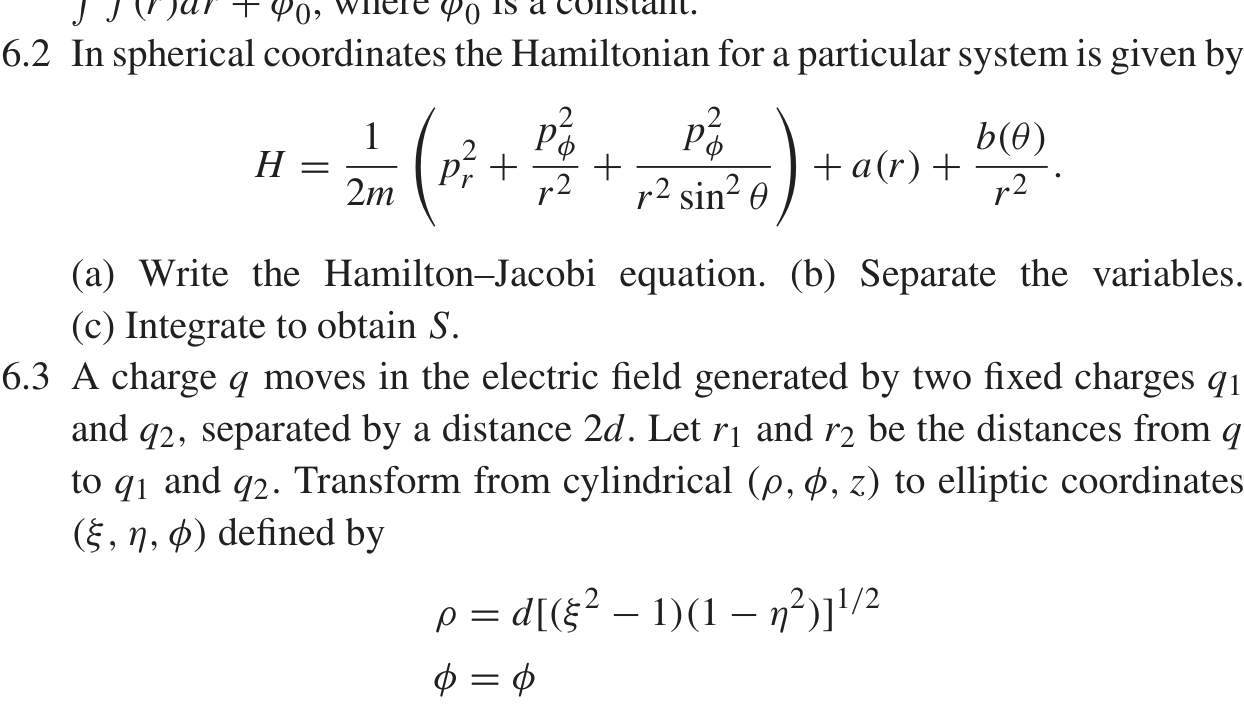
\includegraphics[width=0.55\linewidth]{../Figures/fig_6_1.png}
\caption{Figure 6.1}
\end{figure}

Hamiltonian in terms of p and \textbackslash{}phi , where p is the generalized momentum
and \textbackslash{}phi  is the angular position of the bead relative to the hoop diameter,

6.5
Problems
as shown. (a) Obtain Hamilton's principal function. (b) Obtain an integral
expression for \textbackslash{}phi (t).
6.5 We have expressed Hamilton's principal function as S(qi, \textbackslash{}alpha i, t). Show
that pi, qi, are canonical variables, recalling that
pi = \textbackslash{}partial S
\textbackslash{}partial qi
,
qi = qi(\textbackslash{}alpha , \textbackslash{}beta , t),
where
\textbackslash{}beta i = Qi = \textbackslash{}partial S
\textbackslash{}partial \textbackslash{}alpha i
,
and
\textbackslash{}alpha i = Pi.
\section*{6.6  A particle of mass m is thrown vertically upward in a constant gravitational}

field. Solve the problem of the motion of the particle using the Hamilton--
Jacobi method.
y
z
w
f
wt
A bead on a hoop rotating at constant speed in the horizontal plane.

So far, we have been studying discrete systems, that is, the mechanics of systems that are composed of a collection of particles (or rigid bodies that can be
treated as particles). It is true that, from an atomistic point of view, all mechanical systems can be considered collections of particles. Nevertheless, from a
computational point of view, it is much more convenient to consider some systems as continuous distributions of matter described by continuous properties,
such as the mass density.
When applying variational methods to continuous systems it is convenient
to introduce the Langrangian density L and the Hamiltonian density H. These
can be thought of as the Lagrangian or Hamiltonian per unit volume. The
techniques we shall develop can be applied to a number of different continuous physical systems, and lead nicely into considerations of field theory.
Although we mentioned it in Chapter 1, we have not emphasized the fact
that the Lagrangian is defined to be a function that generates the equations
of motion using the prescription
dt
\textbackslash{}partial L
\textbackslash{}partial $\textbackslash{}dot q$ -\textbackslash{}partial L
\textbackslash{}partial q = 0
or an equivalent relation as determined by the Euler--Lagrange analysis. (That
is, by applying Hamilton's principle.) The fact that L = T -V for particle
mechanics is secondary, although up to this point we have assumed that form
for the Lagrangian.
\section*{7.1  A string}

We begin our consideration with a very simple example of a continuous system, namely a string that is stretched between two end points (denoted